%!TEX root = ../thesis.tex

\section{背景}
近年, 機械学習を用いた自律走行に関する研究が盛んにされており, その中でカメラ画像を用いる研究もされている. Bojarskiら\cite{bojarski}は\figref{Fig:bojarski_train}に示すシステムで, 人間のドライバーが操作するステアリング角度と前方カメラ画像を用いて模倣学習を行った. 加えて, \figref{Fig:bojarski_test}に示すように, 訓練したネットワークに画像を入力し, 生成される操舵指令を用いて走行を行う手法を提案した.

\vspace{0.5cm}

\begin{figure}[hbtp]
  \centering
 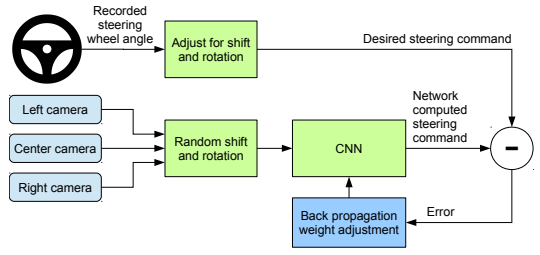
\includegraphics[keepaspectratio, scale=0.9]
      {images/bojarski_train.png}
 \caption{Training the neural network from \cite{bojarski}}
 \label{Fig:bojarski_train}
\end{figure}

\begin{figure}[hbtp]
     \centering
    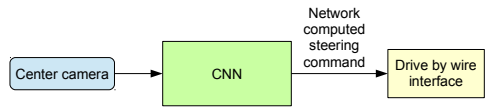
\includegraphics[keepaspectratio, scale=0.7]
         {images/bojarski_test.png}
    \caption{The trained network is used generate steering commands from a single front-facing center camera from \cite{bojarski}}
    \label{Fig:bojarski_test}
\end{figure}

また, \figref{Fig:bojarski_viz}はCNNが人間のドライバーが操作するステアリング角度を教師信号として, 単独で有用な道路の特徴を検出するように学習したことを示している. なお, 道路の輪郭を検出するように明示的に学習をさせていない.

\begin{figure}[hbtp]
     \centering
    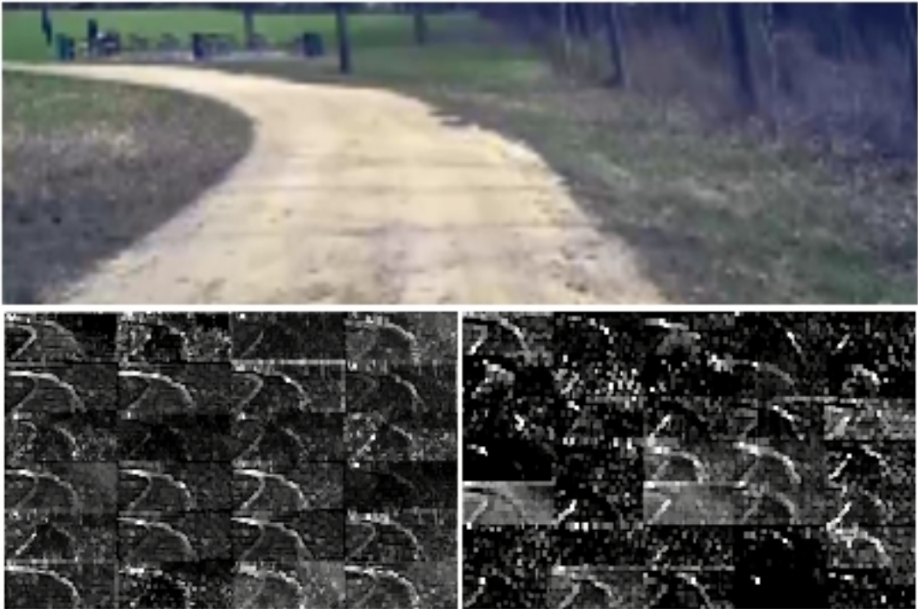
\includegraphics[keepaspectratio, scale=0.3]
         {images/bojarski_viz.png}
    \caption{How the CNN “sees” an unpaved road. Top: subset of the camera image sent to the CNN.
    Bottom left: Activation of the first layer feature maps. Bottom right: Activation of the second layer
    feature maps.  from \cite{bojarski}}
    \label{Fig:bojarski_viz}
\end{figure}


\newpage

本研究室においても, 岡田ら\cite{okada1}\cite{okada2}は\figref{Fig:okada_structure}に示すようなシステムを用いて\figref{Fig:okada_nav}のように経路追従行動を模倣学習し, カメラ画像に基づいた経路追従行動を獲得した. このシステムでは, LiDAR, オドメトリを入力としたルールベース制御器(後述する”地図を用いたルールベース制御器”)による経路追従行動を前方カメラ画像を用いてend-to-endで模倣学習した. 

\vspace{1.5cm}

\begin{figure}[hbtp]
     \centering
     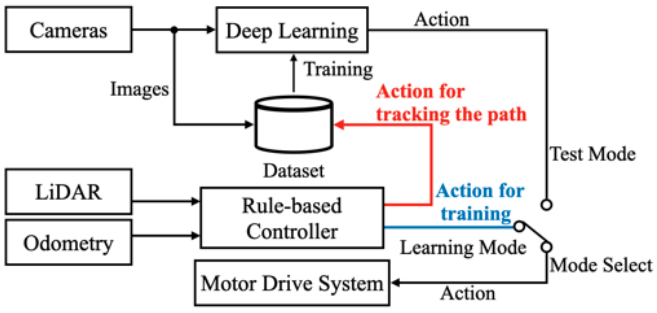
\includegraphics[keepaspectratio, scale=0.55]
          {images/okada_structure.png}
     \caption{Structure of the proposed system from \cite{okada1}}
     \label{Fig:okada_structure}
\end{figure}

\begin{figure}[hbtp]
     \centering
    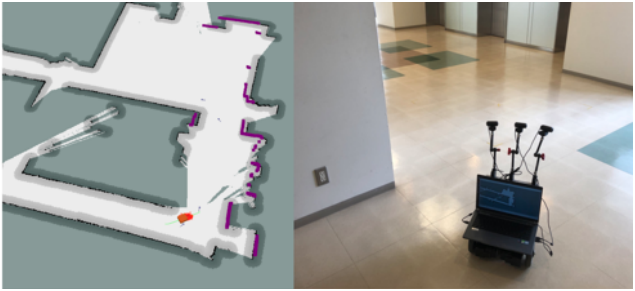
\includegraphics[keepaspectratio, scale=0.5]
         {images/okada_nav.png}
    \caption{A robot that follows a path using vision based on the proposed method from \cite{okada1}}
    \label{Fig:okada_nav}
\end{figure}

\newpage

上記の研究により, カメラ画像に基づいてロボットが学習した経路を周回可能であることが確認されている. 次に岡田らの研究(以下, 「従来手法」と称する)をベースに, \figref{Fig:road}のような分岐路において, 任意の経路を選択する機能の追加を検討する.

\vspace{1cm}

\begin{figure}[hbtp]
     \centering
    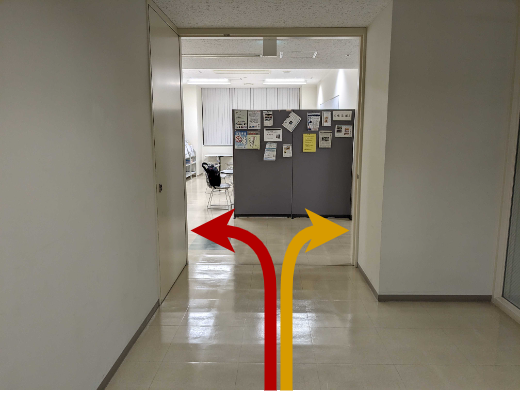
\includegraphics[keepaspectratio, scale=0.5]
         {images/road.png}
    \caption{A fork in the road where the direction of travel is not unique}
    \label{Fig:road}
\end{figure}

\newpage

本研究では, 従来手法をベースに「直進」, 「左折」, 「右折」の目標とする進行方向の情報(以下, 「目標方向」と称する)をデータセットと学習器へ与える. これにより, 訓練済みの学習器の出力を用いた走行において, 目標方向により任意の経路を選択可能とする機能の追加を提案する. 提案手法全体の流れを\figref{Fig:suggest_work}に示す. 

\begin{figure}[hbtp]
     \centering
    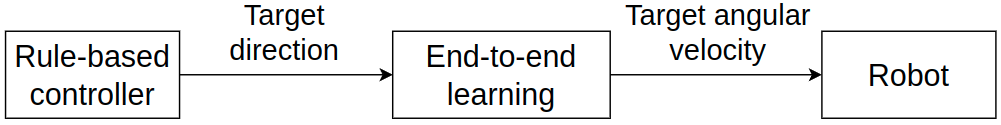
\includegraphics[keepaspectratio, scale=0.38]
         {images/suggest_work.png}
    \caption{Overall flow of the proposed method}
    \label{Fig:suggest_work}
\end{figure}

最終的にはカメラ画像を入力として, トポロジカルマップによって生成される目標方向に従って, 目的地まで移動する自律走行の手法を提案することを検討する. トポロジカルマップとは\figref{Fig:tsudanuma}に示すように, 分岐路などの目印(ノード)とつながり(エッジ)を持つ簡略化された地図である.

\vspace{0.5cm}

\begin{figure}[hbtp]
     \centering
    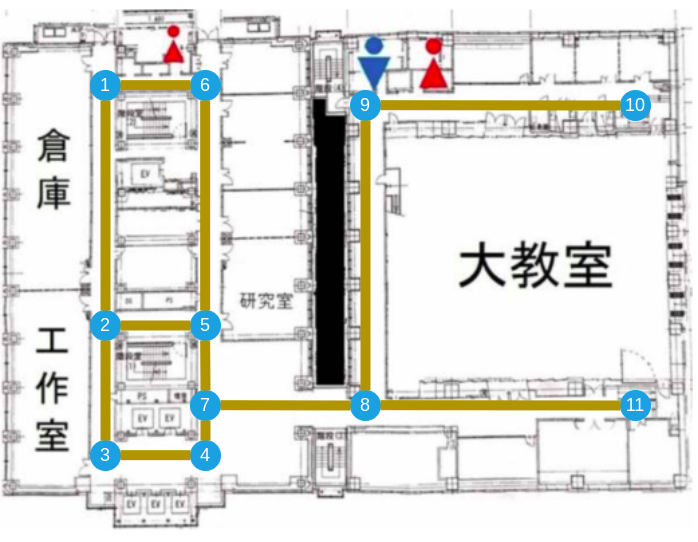
\includegraphics[keepaspectratio, scale=0.45]
         {images/tsudanuma.png}
    \caption{Topological map}
    \label{Fig:tsudanuma}
\end{figure}

カメラ画像とステアリング角度に, 条件を加えて学習を行う条件付き模倣学習
の研究は, 現在までにいくつか行われている.
% によって, 自律移動を行う研究を述べる.
Felipeら\cite{felipe}は前方カメラ画像, ステアリング角度, 加速度と「continue」, 「left」, 「straight」, 「right」からなるコマンドを入力とした\figref{Fig:felipe_network}のようなネットワークを用いて, \figref{Fig:felipe}に示すような実環境と都市環境のシミュレータ上で, 模倣学習のテスト時においてもコマンドによって制御可能であることを確認している.

\vspace{0.5cm}

\begin{figure}[hbtp]
     \centering
    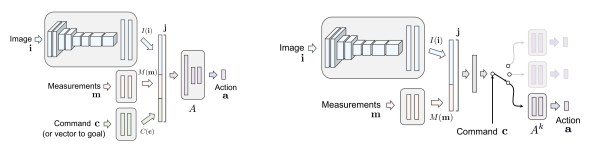
\includegraphics[keepaspectratio, scale=0.65]
         {images/felipe_network.png}
    \caption{Two network architectures for command-conditional imitation learning from \cite{felipe}}
    \label{Fig:felipe_network}
\end{figure}

\vspace{0.5cm}

\begin{figure}[hbtp]
     \centering
    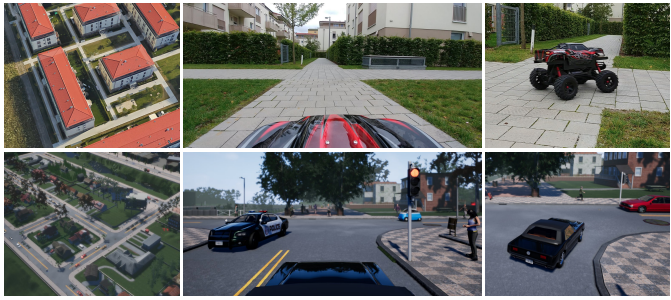
\includegraphics[keepaspectratio, scale=0.57]
         {images/felipe.png}
    \caption{End-to-end driving via conditional imitation learning from \cite{felipe}}
    \label{Fig:felipe}
\end{figure}

\newpage

また, Hawkeら\cite{hawke}は\figref{Fig:hawke}のような, 3つの前方カメラ画像と「go-straight」, 「turn-left」, 「turn-right」からなるコマンドを入力とする構造のモデルを用いて, 実環境での複雑な都市環境というシナリオで, 意思決定が可能なモデルをわずか30時間の学習データで学習可能であることを示している.
だたし, これらの研究は, 本研究の提案するオンラインで自動的にデータセットを収集して学習する仕組みを持っておらず, その点で異なる手法であるといえる.

\vspace{3cm}

\begin{figure}[hbtp]
     \centering
    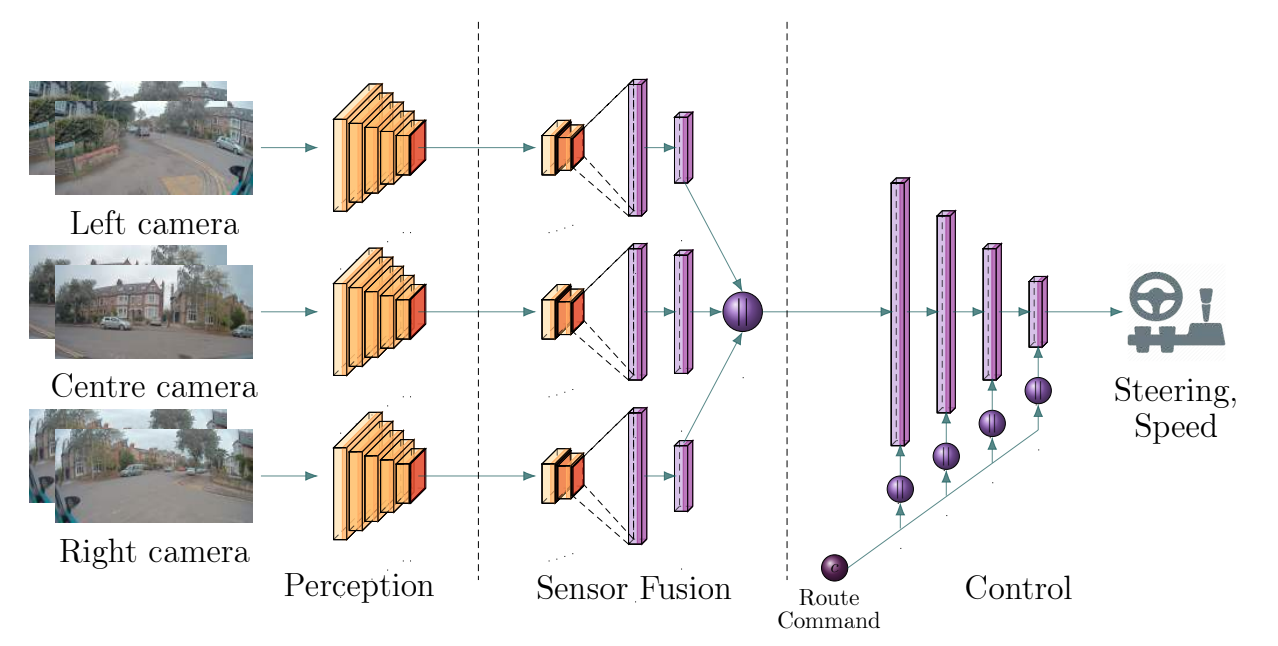
\includegraphics[keepaspectratio, scale=0.3]
         {images/hawke.png}
    \caption{Model structure from \cite{hawke}}
    \label{Fig:hawke}
\end{figure}

\newpage